\chapter{Shape, Position, and Outliers}

Two classes take the same test. Both have a mean score of 75, yet in one class almost everyone scored between
70 and 80, while the other has a cluster of A's and a long tail of failing grades. You scored 85: is that
impressive? It depends on the shape of the scores and on where your score sits among them. In the Numerical
Methods of Describing Data chapter, you learned to measure center and spread. This chapter shows how the
shape of a distribution changes which measures you should trust, and how to describe the position of a
single value with $z$-scores, percentiles, and quartiles.

\section{Connecting Shape to Numerical Measures}

You already know how to read shape from a histogram or boxplot. This
section translates what you see graphically into numerical consequences:
specifically, what skew and outliers do to the measures you just
computed.

\subsection{Symmetric Data: Mean Approximately Equals Median}

When a distribution is roughly symmetric, the mean and median land
close to each other. Neither tail is pulling the mean away from the
center of the data. This is the situation where mean and standard
deviation are both appropriate, and where most inferential procedures
work as intended.


\begin{center}
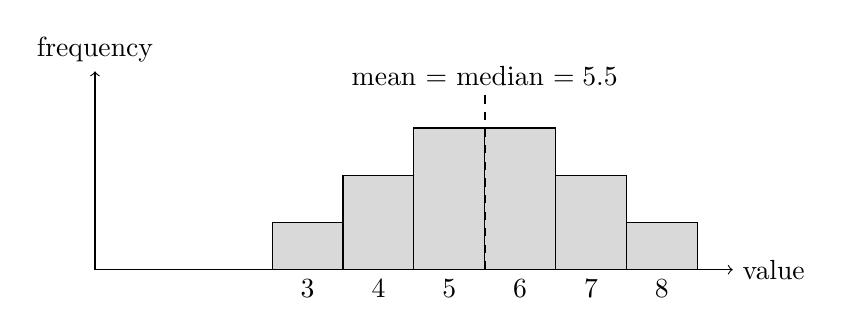
\begin{tikzpicture}[x=0.9cm, y=0.6cm]
    \draw[->] (0,0) -- (9,0) node[right] {value};
    \draw[->] (0,0) -- (0,4.2) node[above] {frequency};
    \foreach \x/\f in {3/1, 4/2, 5/3, 6/3, 7/2, 8/1} {
        \draw[fill=gray!30] (\x-0.5,0) rectangle (\x+0.5,\f);
    }
    \foreach \x in {3,4,5,6,7,8} {
        \node[below] at (\x,0) {\x};
    }
    \draw[thick, dashed] (5.5,0) -- (5.5,3.7);
    \node[above] at (5.5,3.7) {mean = median $= 5.5$};
\end{tikzpicture}

A roughly symmetric data set: $3,\ 4,\ 4,\ 5,\ 5,\ 5,\ 6,\ 6,\ 6,\ 7,\
7,\ 8$. The mean and median land at exactly the same value.
\end{center}

\subsection{Skewed Data: Mean Pulled Toward the Tail}

When a distribution is skewed, the mean chases the tail while the
median stays near the bulk of the data. The direction of the skew
tells you exactly which way the mean is pulled:

\begin{center}
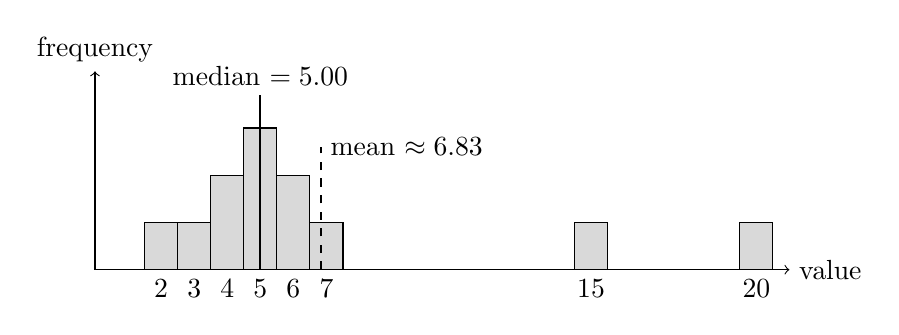
\begin{tikzpicture}[x=0.42cm, y=0.6cm]
    \draw[->] (0,0) -- (21,0) node[right] {value};
    \draw[->] (0,0) -- (0,4.2) node[above] {frequency};
    \foreach \x/\f in {2/1, 3/1, 4/2, 5/3, 6/2, 7/1, 15/1, 20/1} {
        \draw[fill=gray!30] (\x-0.5,0) rectangle (\x+0.5,\f);
    }
    \foreach \x in {2,3,4,5,6,7,15,20} {
        \node[below] at (\x,0) {\x};
    }
    \draw[thick] (5,0) -- (5,3.7);
    \node[above] at (5,3.7) {median $=5.00$};
    \draw[thick, dashed] (6.83,0) -- (6.83,2.6);
    \node[right] at (6.83,2.6) {mean $\approx 6.83$};
\end{tikzpicture}

The right-skewed data set below: two extreme values at 15 and 20
pull the mean well past the median.
\end{center}

\begin{itemize}
    \item Right-skewed: mean $>$ median. The right tail pulls the
    mean upward.
    \item Left-skewed: mean $<$ median. The left tail pulls the mean
    downward.
\end{itemize}

This pattern follows directly from what you already know about the
mean. Because the mean uses every value in its calculation, a cluster
of extreme values in the right tail will drag it rightward. The median, which depends only on rank order, does not
move.

Consider a small right-skewed data set:

\[ 2,\ 3,\ 4,\ 4,\ 5,\ 5,\ 5,\ 6,\ 6,\ 7,\ 15,\ 20 \]

The mean is approximately 6.83 and the median is 5.00. The two extreme
values at 15 and 20 pull the mean well above where most of the data
sits. On a histogram, most bars would be clustered at the left with a
long right tail. This shape corresponds to mean $>$
median.

\subsection{Effects of Outliers}

An \newterm{outlier}\index{outlier} is a value that sits far from the
rest of the data. You saw the numerical definition in the graphical
chapter: any value more than $1.5 \times IQR$ below $Q_1$ or above
$Q_3$ is flagged as an outlier.

What outliers do to each measure follows directly from whether that
measure is resistant:

\begin{itemize}
    \item Mean: pulled toward the outlier. One extreme value can move
    the mean substantially.
    \item Median: unaffected. Moving the most extreme value further
    into the tail does not change the middle rank.
    \item Standard deviation: inflated. Because it is computed from
    the mean, an outlier that moves the mean also increases the
    squared deviations.
    \item IQR: unaffected. It depends only on $Q_1$ and $Q_3$, which
    are determined by the middle of the data.
\end{itemize}

This is why mean and standard deviation always travel together, and
median and IQR always travel together. They are basically matched pairs.

\subsection{Changing Units on Summary Measures}

One practical question comes up often: if every value in a data set
is shifted or scaled, what happens to the summary measures? Suppose a
teacher adds 20 points to every student's test score, or a government
increases all property taxes by 2\%. You do not need to recompute
everything from scratch.

The rules depend on whether you are adding a constant or multiplying
by one.

\index{linear transformation}\textbf{Adding a constant $a$ to every value.} Shifting every
observation by the same amount shifts the measures of center and
position by the same amount. Measures of spread are unaffected,
because the distances between values do not change.

\textbf{Multiplying every value by a constant $b$.} Scaling every
observation multiplies all measures, such as center, spread, and position, by the same factor. The absolute value $|b|$ is used for
spread measures, since spread is always non-negative.

These rules are summarized in the table below.

\begin{center}
\begin{tabular}{lll}
\textbf{Measure} & $Y_i = X_i + a$ & $Y_i = b \cdot X_i$ \\
\hline
Mean        & $\bar{Y} = \bar{X} + a$     & $\bar{Y} = b\bar{X}$ \\
Median      & Median$(Y)$ = Median$(X) + a$ & Median$(Y) = b \cdot$Median$(X)$ \\
Range       & Unaffected                  & Range$(Y) = |b|$\,Range$(X)$ \\
Std dev     & Unaffected                  & $s_Y = |b| \cdot s_X$ \\
$Q_1$, $Q_3$  & $Q_1 + a$,\ $Q_3 + a$      & $b \cdot Q_1$,\ $b \cdot Q_3$ \\
IQR         & Unaffected                  & $IQR(Y) = |b| \cdot IQR(X)$ \\
\end{tabular}
\end{center}

The key pattern: adding a constant moves everything but changes no
distances; multiplying stretches or compresses everything including
distances.

\textbf{Example.} A class takes a five-question test worth 20 points
each. The summary statistics for their scores are:

\begin{center}
\begin{tabular}{ll}
Mean & 62 \\
Median & 60 \\
Range & 45 \\
Standard deviation & 8 \\
$Q_1$ & 48 \\
$Q_3$ & 71 \\
IQR & 23 \\
\end{tabular}
\end{center}

After grading, the teacher discovers a typographical error in question
2 that made it unanswerable. She adds 20 points to every student's
score. The new summary statistics are:

\begin{center}
\begin{tabular}{lll}
\textbf{Measure} & \textbf{Original} & \textbf{After adding 20} \\
\hline
Mean        & 62 & $62 + 20 = 82$ \\
Median      & 60 & $60 + 20 = 80$ \\
Range       & 45 & 45 (unaffected) \\
Std dev     & 8  & 8 (unaffected) \\
$Q_1$       & 48 & $48 + 20 = 68$ \\
$Q_3$       & 71 & $71 + 20 = 91$ \\
IQR         & 23 & 23 (unaffected) \\
\end{tabular}
\end{center}

Every student's score shifted by the same amount, so the spread of
the distribution is unchanged. The center and quartiles each moved
up by exactly 20.

\begin{Exercise}[title={Changing Units}, label={ex:changing_units}]
County residents vote to increase property taxes by 2\% to fund local
schools. The current summary statistics for property tax (in dollars
per year) are:

\begin{center}
\begin{tabular}{ll}
Mean & 12{,}000 \\
Median & 8{,}000 \\
Range & 30{,}000 \\
Standard deviation & 5{,}000 \\
$Q_1$ & 5{,}000 \\
$Q_3$ & 14{,}000 \\
IQR & 9{,}000 \\
\end{tabular}
\end{center}

Each resident's new tax will be $1.02 \times$ their current tax.
Compute the new value of each summary measure.
\end{Exercise}

\begin{Answer}[ref={ex:changing_units}]
Multiplying every value by $b = 1.02$:

\begin{center}
\begin{tabular}{lll}
\textbf{Measure} & \textbf{Original} & \textbf{After multiplying by 1.02} \\
\hline
Mean        & 12{,}000 & $1.02(12{,}000) = 12{,}240$ \\
Median      & 8{,}000  & $1.02(8{,}000) = 8{,}160$ \\
Range       & 30{,}000 & $1.02(30{,}000) = 30{,}600$ \\
Std dev     & 5{,}000  & $1.02(5{,}000) = 5{,}100$ \\
$Q_1$       & 5{,}000  & $1.02(5{,}000) = 5{,}100$ \\
$Q_3$       & 14{,}000 & $1.02(14{,}000) = 14{,}280$ \\
IQR         & 9{,}000  & $1.02(9{,}000) = 9{,}180$ \\
\end{tabular}
\end{center}

Unlike adding a constant, multiplying affects the spread measures too.
Every distance in the distribution is stretched by the same factor.
\end{Answer}

\section{Z-scores}

The previous section showed that adding a constant to every value
shifts the mean but leaves the standard deviation unchanged. That
means the distances between values, relative to the center, stay
exactly the same. There is a natural way to express those distances
as a single number: the \newterm{z-score}\index{z-score}, also called
a \newterm{standardized score}\index{standardized score}.

The z-score of a measurement tells you how far that value sits from
the mean, expressed in units of standard deviations:

\[
z = \frac{x - \bar{x}}{s}
\]

For population data, replace $\bar{x}$ with $\mu$ and $s$ with
$\sigma$. The interpretation is the same either way.

A positive z-score means the value is above the mean. A negative
z-score means it is below. A z-score of zero means the value equals
the mean exactly. The magnitude tells you how many standard deviations
separate the value from the center.

\textbf{Example.} A class takes a test with mean 74 and standard
deviation 6. Two students receive the following scores:

\begin{center}
\begin{tabular}{lcl}
Amaka & 88 &
$z = \dfrac{88 - 74}{6} = \dfrac{14}{6} \approx 2.33$ \\[10pt]
George & 70 &
$z = \dfrac{70 - 74}{6} = \dfrac{-4}{6} \approx -0.67$ \\
\end{tabular}
\end{center}

Amaka scored about 2.33 standard deviations above the class
average. George scored about 0.67 standard deviations below it.
George is actually closer to the mean than Amaka: $|-0.67|
< |2.33|$.

\subsubsection*{Comparing Across Different Distributions}

Z-scores become especially powerful when comparing measurements from
distributions with different means and standard deviations. Without
standardization, comparing values measured on different scales is
meaningless. With z-scores, it becomes straightforward.

Suppose two cities report their daily high temperatures:

\begin{center}
\begin{tabular}{lcc}
City & Mean daily high & Standard deviation \\
\hline
North Bend & $80^{\circ}$F & $12^{\circ}$F \\
South Bend & $84^{\circ}$F & $4^{\circ}$F \\
\end{tabular}
\end{center}

Both cities report a high of $95^{\circ}$F on the same day. Which
city had the more unusually warm day?

The raw difference from the mean is larger for North Bend
($95 - 80 = 15$) than South Bend ($95 - 84 = 11$), but that ignores
how variable the temperatures are in each city. Compute the z-scores:

\[
\text{North Bend: } z = \frac{95 - 80}{12} = 1.25
\qquad
\text{South Bend: } z = \frac{95 - 84}{4} = 2.75
\]

South Bend's $95^{\circ}$F sits 2.75 standard deviations above its
mean, which is far more unusual than North Bend's 1.25. The day was more
remarkably warm in South Bend, even though it was not further above
South Bend's mean in raw degrees.

\begin{Exercise}[title={Computing and Interpreting Z-scores},
label={ex:zscores}]
Daniel's car dealership from earlier in this chapter had mean daily
sales of $\bar{X} \approx 14.64$ cars and standard deviation $s \approx
7.56$ cars.

\begin{enumerate}  
    \item Compute the z-score for the best sales day (24 cars).
    Interpret it in context.
    \item Compute the z-score for the worst sales day (2 cars).
    Interpret it in context.
    \item A second dealership reports a best day of 31 cars, with
    mean 20 and standard deviation 4. Which dealership had the more
    unusually good best day? Show your work.
    \item Daniel adds a fixed weekend
    bonus, increasing every daily total by 5 cars. Without
    recomputing, what is the z-score for the original best day
    of 24 cars under the new totals? Explain.
\end{enumerate}
\end{Exercise}

\begin{Answer}[ref={ex:zscores}]
\begin{enumerate}  
    \item $z = \dfrac{24 - 14.64}{7.56} \approx 1.24$. The best day
    was about 1.24 standard deviations above the mean. It was a
    notably good day but not extreme.
    \item $z = \dfrac{2 - 14.64}{7.56} \approx -1.67$. The worst day
    was about 1.67 standard deviations below the mean and further from
    typical than the best day was above it.
    \item Second dealership: $z = \dfrac{31 - 20}{4} = 2.75$.
    The second dealership's best day was more unusually high at 2.75
    standard deviations above its mean, compared to 1.24 for the
    first dealership.
    \item Still $z \approx 1.24$. Adding a constant to every value
    shifts the mean by the same constant and leaves the standard
    deviation unchanged. The relative position of every observation
    in the distribution stays the same, so z-scores are unaffected.
\end{enumerate}
\end{Answer}

\textbf{Key points:}
\begin{itemize}
    \item A z-score expresses a value as a number of standard
    deviations above or below the mean
    \item Positive z-scores are above the mean; negative z-scores
    are below it
    \item Z-scores allow meaningful comparison across data sets
    measured on different scales
    \item Adding a constant to every value does not change any
    z-score; z-scores are invariant under shifting
\end{itemize}

\section{Percentiles and Quartiles}

The mean, median, and standard deviation describe the whole
distribution. Sometimes the question is narrower: where does one
particular value sit relative to everyone else? Mary, who scores
1400 on the SAT, wants to know not just that the median was 1040,
but what percentage of students she scored above. That is what
percentiles and quartiles answer.

\subsection*{Percentiles}

The \newterm{$k$th percentile}\index{percentile} $P_k$ is the value
such that $k\%$ of observations fall at or below it and $(100-k)\%$
fall at or above it. For example, $P_{95}$ is the 95th percentile:
a value at $P_{95}$ is higher than 95\% of the data and lower than
the remaining 5\%.

Three percentiles you already know appear here under new names:
$P_{25} = Q_1$, $P_{50} = Q_2 = M$ (the median), and $P_{75} = Q_3$.

To find $P_k$ for a data set of $n$ measurements:

\begin{enumerate}
    \item Arrange all measurements in increasing order.
    \item Compute $l = \dfrac{(n+1)k}{100}$.
    \item $P_k$ is the value of the measurement in position $l$,
    counted from the smallest. If $l$ is not a whole number,
    interpolate between the two surrounding observations.
\end{enumerate}

Return to the dealership data ($n = 14$, sorted):

\[ 2,\ 3,\ 7,\ 9,\ 11,\ 11,\ 14,\ 17,\ 20,\ 20,\ 21,\ 23,\ 23,\ 24 \]

To find $P_{90}$:

\[
l = \frac{(14+1) \times 90}{100} = 13.5
\]

The 90th percentile falls halfway between the 13th and 14th
observations. The 13th is 23 and the 14th is 24:

\[
P_{90} = \frac{23 + 24}{2} = 23.5 \text{ cars}
\]

Roughly 90\% of days fall at or below 23.5 cars. (With only 14 days, the
match is not exact: 12 of the 14 days, about 86\%, are at or below
23.5.)

To find $P_{10}$:

\[
l = \frac{(14+1) \times 10}{100} = 1.5
\]

Halfway between the 1st observation (2) and the 2nd (3):

\[
P_{10} = \frac{2 + 3}{2} = 2.5 \text{ cars}
\]

Roughly 10\% of days fall at or below 2.5 cars.

\subsection*{Quartiles and the Five-Number Summary}

\newterm{Quartiles}\index{quartiles} divide a sorted data set into
four equal parts using the 25th, 50th, and 75th percentiles. You
first encountered these when building boxplots in the \textit{Introduction to Data Visualization}
chapter. Here is the formal connection:

\begin{itemize}
    \item $Q_1 = P_{25}$: 25\% of values fall at or below $Q_1$
    \item $Q_2 = P_{50} = M$: the median
    \item $Q_3 = P_{75}$: 75\% of values fall at or below $Q_3$
\end{itemize}

\index{quartiles!median-of-halves method}In practice, quartiles are computed by splitting the sorted data into
a lower half and an upper half and taking the median of each. For
even $n$, split the data at the midpoint with no overlap. For odd
$n$, exclude the median from both halves.


For the dealership data, split at the midpoint ($n = 14$, so seven
values on each side):

\begin{center}
Lower half: $2,\ 3,\ 7,\ \mathbf{9},\ 11,\ 11,\ 14$
$\Rightarrow Q_1 = 9$ \\[4pt]
Upper half: $17,\ 20,\ 20,\ \mathbf{21},\ 23,\ 23,\ 24$
$\Rightarrow Q_3 = 21$
\end{center}

You may notice that the median-of-halves method gives $Q_1 = 9$,
while the percentile formula gives $P_{25} = 8.5$. Both are correct, as different software and textbooks use slightly different conventions
for quartile computation. Small disagreements between methods are
normal and expected. On the AP exam, the median-of-halves method is
standard.

Together with the minimum and maximum, the quartiles form the
\newterm{five-number summary}\index{five-number summary}: the same
five values you used to build a boxplot.

\begin{center}
\begin{tabular}{lllll}
Min & $Q_1$ & Median & $Q_3$ & Max \\
\hline
2 & 9 & 15.5 & 21 & 24 \\
\end{tabular}
\end{center}

The five-number summary and the boxplot are two representations of
exactly the same information: one numerical, one graphical.

\begin{Exercise}[title={Relative Standing},
label={ex:percentiles}]
Use the dealership data: \\
$2,\ 3,\ 7,\ 9,\ 11,\ 11,\ 14,\ 17,\ 20,\ 20,\ 21,\ 23,\ 23,\ 24$
($n = 14$).

\begin{enumerate}  
    \item Compute $P_{50}$ using the formula $l = \dfrac{(n+1)k}{100}$.
    Does it match the median you computed earlier? What position in
    the sorted list does $l$ point to?
    \item On what percentage of days did the dealership sell at most
    21 cars?
    \item A sales consultant tells Daniel that a day with 17 cars
    sold falls in the ``third quarter'' of the distribution. Verify
    this by identifying which quarter 17 belongs to.
    \item Daniel wants to flag the bottom 10\% of days as
    underperforming. Using $P_{10} = 2.5$ cars, how many of the 14
    days fall in this category? List them.
\end{enumerate}
\end{Exercise}

\begin{Answer}[ref={ex:percentiles}]
\begin{enumerate}  
    \item $l = \dfrac{(14+1)(50)}{100} = 7.5$. The 50th percentile
    falls halfway between the 7th observation (14) and the 8th (17):
    $P_{50} = \dfrac{14+17}{2} = 15.5$. This matches the median
    exactly.
    \item Count them: 11 of the 14 days had 21 or fewer cars, so
    $\frac{11}{14} \approx 79\%$. (Since $Q_3 = 21$, you could also
    estimate about 75\%; with small data sets the quartiles are only
    approximate percentages.)
    \item $Q_1 = 9$ and $Q_3 = 21$. The value 17 lies between $Q_2
    = 15.5$ and $Q_3 = 21$, placing it in the third quarter (between
    the median and $Q_3$). The consultant is correct.
    \item Days with 2 or fewer cars: only the day with 2 cars sold.
    That is 1 out of 14 days, or about 7\%, consistent with
    the bottom 10\% cutoff of 2.5.
\end{enumerate}
\end{Answer}

\subsection{Computing with Python}

You have now computed measures of center, spread, and position by
hand. In practice, you will
rarely compute them this way. Python's built-in \texttt{statistics}
module handles all of them directly, using the dealership data set
from throughout this chapter:

% corresponding script: computing_with_python.py
\begin{minted}{python}
import statistics

sales = [14, 9, 23, 7, 11, 23, 17, 11, 3, 24, 21, 2, 20, 20]

print("mean:    ", statistics.mean(sales))
print("median:  ", statistics.median(sales))
print("variance:", round(statistics.variance(sales), 2))
print("stdev:   ", round(statistics.stdev(sales), 2))

q1, q2, q3 = statistics.quantiles(sales, n=4)
print("Q1, Q2, Q3:", q1, q2, q3)
\end{minted}

This prints a mean of 14.642857142857142, a median of 15.5, a
variance of 57.17, and a standard deviation of 7.56, matching this
chapter's hand-computed values. The quartiles come out as 8.5, 15.5, and
21.5: \texttt{statistics.quantiles} uses the percentile formula, not the
median-of-halves method, which is why its $Q_1$ and $Q_3$ differ slightly
from ours.



